\Transcb{yellow}{blue}{Effects in a uniform gravitational field}
\onecolumn
\begin{center}
{\blue Gravitational time dilation}
\end{center}
\begin{itemize}
\item Consider a rocket in empty space with constant vertical acceleration $g\,\hat{z}$
\item[] Nose of the rocket~: Observer A with clock A emitting light signals at intervals $\Delta\tau_{A}$
\item[] Tail of the rocket~: Observer B with clock B receiving light signals at intervals $\Delta\tau_{B}$
\item[$\ast$] Distance A-B $\equiv h$~: {\red At what time intervals does observer B receive the signals~?}
\end{itemize}
%
\begin{center}
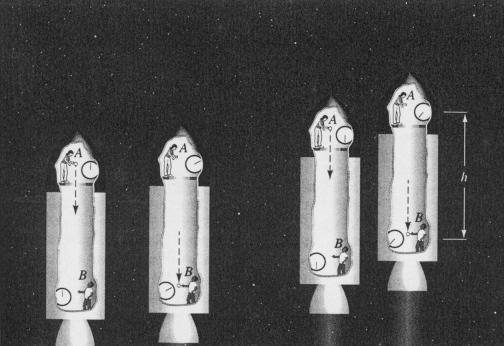
\includegraphics[keepaspectratio,height=9cm]{clocks}
\end{center}

\Tr
\begin{itemize}
\item Enable simple Newtonian mechanics by selecting an inertial frame such that
\item[] $V \ll c$ ($V$ is rocket velocity at signal emission) $\rightarrow$ non-relativistic
\item[] $gh/c \ll c \rightarrow$ No acceleration to relativistic $V$ while light travels nose-tail
\item Choose origin of time~: First pulse emitted at $t=0$ and $z_{B}(t=0) \equiv 0$
\item[] $V(t=0) \equiv 0 \rightarrow$ Observer locations~:
        {\blue $z_{B}(t)=\frac{1}{2}gt^{2} \qquad z_{A}(t)=h+\frac{1}{2}gt^{2}$}
\item[] First pulse received at $t=t_{1} \qquad$ second pulse emitted at $t=\Delta\tau_{A}$
\item[] and second pulse received at $t=t_{1}+\Delta\tau_{B}$
\item Approximation which is accurate to leading order in $gh/c^{2}$~:
\item[] Distance traveled by first pulse~: $z_{A}(0)-z_{B}(t_{1})=ct_{1}$
\item[] Distance traveled by second pulse~:
        $z_{A}(\Delta\tau_{A})-z_{B}(t_{1}+\Delta\tau_{B})=c(t_{1}+\Delta\tau_{B}-\Delta\tau_{A})$
\item[] Using the observer locations and neglecting higher orders of $\Delta\tau_{A}$ and $\Delta\tau_{B}$~:
\item[] $\quad h-\frac{1}{2}gt_{1}^{2}=ct_{1} \quad \text{and} \quad
        h-\frac{1}{2}gt_{1}^{2}-gt_{1}\Delta\tau_{B}=c(t_{1}+\Delta\tau_{B}-\Delta\tau_{A})$
\item[] $\rightarrow \displaystyle {\blue \Delta\tau_{B}} =\frac{c\Delta\tau_{A}}{c+gt_{1}}
         \approx \frac{c\Delta\tau_{A}}{c+gh/c} {\blue = \frac{\Delta\tau_{A}}{1+gh/c^{2}}}$
\end{itemize}

\Tr
\twocolumn[\begin{center}
           {\red Equivalence principle~: The same must happen in a uniform gravitational field}
           \vspace*{3mm}
           \end{center}]
%
\begin{itemize}
\item {\blue Gravitational time dilation}
\item[] $\displaystyle \Delta\tau_{B} \approx \frac{\Delta\tau_{A}}{1+gh/c^{2}}$
\item[] {\blue Emission and reception rates $\nu$}~: 
\item[] $\nu_{B} \approx \nu_{A}\,(1+gh/c^{2})$
\item In terms of the {\blue gravitational potential $\Phi$}~:
\item[] {\red \shabox{$\displaystyle \nu_{B} \approx \nu_{A}\left(1+\frac{\Phi_{A}-\Phi_{B}}{c^{2}}\right)$}}
\item[] Also valid in non-uniform grav. fields
\item[] \begin{center}\colorbox{yellow}{Gravitational red shift}\end{center}
\item[] {\blue $\displaystyle z \equiv \frac{\lambda_{obs}-\lambda_{emit}}{\lambda_{emit}}
         =\frac{\lambda_{obs}}{\lambda_{emit}}-1$}
\item[] ($z<0 \rightarrow$ blue shift)
\end{itemize}

\newpage
%
\begin{center}
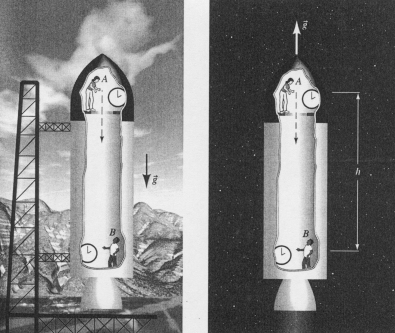
\includegraphics[keepaspectratio,height=9.5cm]{clocks2}
\end{center}
%
\begin{itemize}
{\red
\item[$\ast$] Exercise~: Determine the redshift at\\
              $r=\infty$ for the light emitted from the edge 
              of a white dwarf with mass $M=M_{\odot}$ and radius $R=10^{3}$~km
}
\end{itemize}

\Tr
\onecolumn
\begin{center}
{\blue Gravitational deflection of light}
\end{center}
\begin{itemize}
\item Consider a rocket in empty space with constant vertical acceleration $g\,\hat{z}$
\item[] Light ray enters (upper window) and exits (lower window)
\item[] Outside inertial frame~: light ray describes straight path
\item[] Accelerated rocket frame~: light ray falls down with acceleration $g$
\end{itemize}
%
\begin{center}
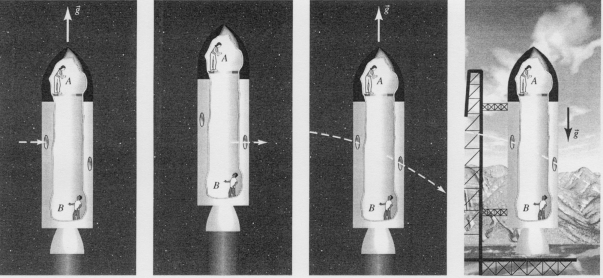
\includegraphics[keepaspectratio,height=8.5cm]{light}\\
\colorbox{yellow}{A light ray in a gravitational field must fall with the same acceleration as other objects} 
\end{center}
%
